\documentclass[tikz,border=10pt]{standalone}
\usetikzlibrary{calc}
% Scale s = 0.012719 cm/px; origin = ink bbox centre (352, 159.5) px, y flipped
\begin{document}
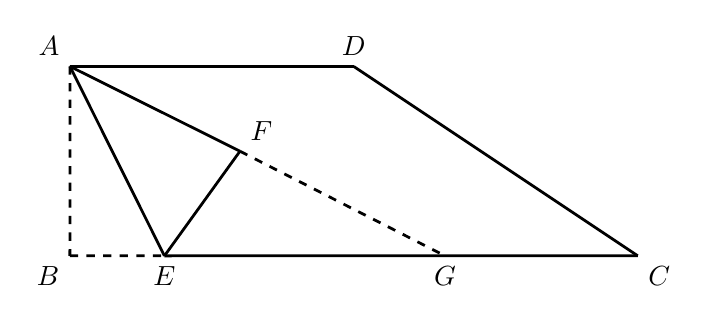
\begin{tikzpicture}[line width=1.0pt, line join=round,
  lbl/.style={font=\fontsize{10}{12}\selectfont}]
  % Named coordinates (cm)
  \coordinate (A) at (-3.605,  1.203);
  \coordinate (B) at (-3.606, -1.202);
  \coordinate (C) at ( 3.606, -1.202);
  \coordinate (D) at ( 0.000,  1.202);
  \coordinate (E) at (-2.405, -1.203);
  \coordinate (F) at (-1.446,  0.126);
  \coordinate (G) at ( 1.157, -1.202);

  % Solid: top line, slanted lines
  \draw (A) -- (D);
  \draw (D) -- (C);
  \draw (A) -- (E);
  \draw (A) -- (F);
  \draw (E) -- (F);
  % Bottom line: solid part E--C (B--E is dashed)
  \draw (E) -- (C);

  % Dashed: vertical A--B, bottom-left B--E, F--G
  \draw[dashed] (A) -- (B);
  \draw[dashed] (B) -- (E);
  \draw[dashed] (F) -- (G);

  % Labels
  \node[lbl, above left]  at (A) {$A$};
  \node[lbl, below left]  at (B) {$B$};
  \node[lbl, below right] at (C) {$C$};
  \node[lbl, above]       at (D) {$D$};
  \node[lbl, below]       at (E) {$E$};
  \node[lbl, above right] at (F) {$F$};
  \node[lbl, below]       at (G) {$G$};
\end{tikzpicture}
\end{document}